\documentclass[oneside,a4paper,12pt]{article}
\usepackage{graphicx}
\usepackage[section]{placeins}
\usepackage{listings}
\graphicspath{{~/templates/}, {../images/}}

\makeindex
\begin{document}
	\begin{titlepage}
		\includegraphics[width=4cm]{logopopo.png}
		\hspace*{\fill}
		\includegraphics[width=6cm]{univlille.png}
		
		\begin{center}
			\vspace{1cm}
			\textbf{TP Variation de Vitesse}\\
			\textbf{TP1 }\\
			\vspace{1cm}
			\textbf{Valentin DOSIAS, Maxence NEUS}\\
			\vspace{3cm}
			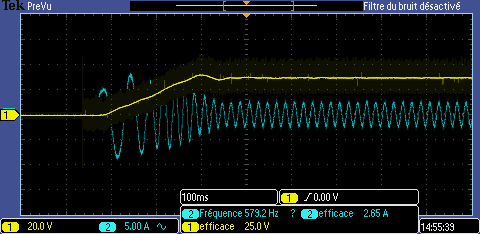
\includegraphics[width=13cm]{titlepage.png}\\
			\vspace{\fill}
			\textbf{Novembre 2021}\\
		\end{center}
	\end{titlepage}
	
	\tableofcontents
	\newpage
	
	\section{Introduction}
	
	L’objectif de ce TP est de mettre en évidence les interactions qui existent entre un entraînement à vitesse variable et sa charge. On montre ainsi que le choix d’un entraînement à vitesse variable ne peut s’effectuer sans prise en compte des caractéristiques mécaniques de la charge.\\
	Pour ce faire, nous allons utiliser la machine asynchrone représentant la motorisation qui va entraîner la machine à courant continu représentant une charge variable.\\
	Nous allons comparer deux modes d'entraînement à vitesse variable pour cette machine. Le premier mode consiste à ajuster la tension d’alimentation en gardant une fréquence constante. Le second mode consiste à faire varier la fréquence d’alimentation en gardant le rapport tension/fréquence d’alimentation constant. Les deux systèmes seront étudiés à vide et en charge. La caractéristique couple/vitesse ainsi que le comportement en régime transitoire de chacun des deux modes de fonctionnement sera étudiés.\\
	
	\section{Préparation}
	
	La préparation est disponible en annexe.
	
	\section{Manipulations}
	
	Pour ce tp nous avons travaillé avec un tachymètre qui délivre 20V pour 1000tr/min.\\
	
	\subsection{Commande en tension simple}
	
	Nous alimentons d’abord la machine asynchrone avec une tension entre phases U=380V, nous mesurons le courant d’induit de la machine à courant continu et le courant absorbé par la machine asynchrone.\\
	Nous réitérons les relevés pour une tension entre phases de 190V toujours en faisant attention à ne pas dépasser le courant nominal de la machine asynchrone qui est de 3.4A.\\
	On alimente l’inducteur sous 190V. Pour cette alimentation, l’énoncé nous donne 
	$$ k_{\Phi}=1.15 V.(rad.s^{-1})^{-1}$$
	Nous obtenons donc les caractéristiques couple/vitesse suivante : \\
	
	\begin{figure}[h]
		\centering
		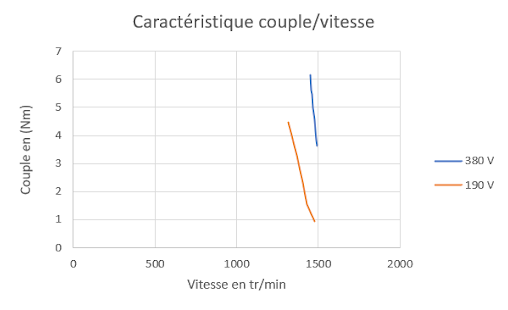
\includegraphics[width=12cm]{couple_vitesse1.png}
		\caption{Caractéristique couple/vitesse}
	\end{figure}
	
	Nous obtenons bien deux courbes l’une en dessous de l’autre comme dans la préparation. Les courbes sont cohérentes, plus l’on approche de la vitesse de synchronisme plus le couple baisse. Les courbes ne semble pas être parallèle, si on les prolonge, théoriquement elles se croiseraient au point (1500,0).\\
	Pour  U=380 V, nous ne pouvons pas descendre plus bas en vitesse car nous sommes limités en charge (max : 2100 W). Pour U= 190 V, nous ne pouvons pas augmenter la charge car sinon la machine asynchrone absorbe plus que son courant nominal (3.4 A).\\
	Dans la préparation nous avons calculé qu’il que pour entraîner l’ascenseur soit 300kg de charge, il faut que la machine délivre un couple supérieur à 3 Nm. Si l’on alimente la machine avec 190 V entre phases, il faut que la vitesse du moteur soit entre 1350 tr/min pour développer assez de couple et 1300 tr/min pour respecter le courant nominal de la machine. Pour l’alimentation de 380V, entre 1450 et 1490 tr/min la machine délivre un couple supérieur à 3 Nm, elle peut donc entraîner l’ascenseur.\\
	
	\subsection{Commande en V/f avec le variateur}
	
	Nous allons maintenant alimenter la machine asynchrone par un variateur électronique. Ce variateur permet de faire varier la fréquence d’alimentation de la machine en conservant le rapport V/f constant. 
	Le potentiomètre indique un pourcentage de la fréquence d'alimentation soit théoriquement 50Hz.\\
	
	\paragraph{Visualisation des formes d'ondes}\paragraph{}
	
	Nous avons d’abord visualisé  le courant et la tension aux bornes de la machine sans le filtre RC. Nous voyons alors des pics de tensions liés aux commutations des transistors du variateur, nous voyons la tension découpée par le variateur.\\
	Nous utilisons un filtre RC pour ne garder que le fondamental de la tension et avoir des valeurs plus précises pour nos mesures. Nous avons observé un déphasage entre la tension et le courant lié au système inductif de la machine asynchrone. Nous avons fait nos relevés avec le filtre.\\
	Nous obtenons les valeurs suivantes : \\
	\begin{figure}[h]
		\begin{center}
			\begin{tabular}{|p{0.2\textwidth}|p{0.2\textwidth}|p{0.2\textwidth}|p{0.2\textwidth}|p{0.2\textwidth}|}
				\hline
				\% du potentiomètre & Periode mesurée de ms & Fréquence mesurée & Tension d'alimentation mesurée & Rapport V/f\\
				\hline
				\hline
				20 & 120 & 8.33 & 49 & 5.88\\ 
				\hline
				30 & 71.2 & 14.05 & 86.9 & 6.19\\ 
				\hline
				40 & 52 & 19.23 & 125 & 6.5\\ 
				\hline
				50 & 40 & 25 & 166 & 6.64\\ 
				\hline
				60 & 33 & 30.3 & 203 & 6.699\\ 
				\hline
				70 & 28 & 35.7 & 250 & 7\\ 
				\hline
				80 & 23.8 & 42.02 & 289 & 6.88\\ 
				\hline
				90 & 20.8 & 48.08 & 331 & 6.88\\
				\hline
				100 & 20 & 50 & 337 & 6.74\\ 
				\hline
			\end{tabular}
		\end{center}
		\caption{Mesures du rapport V/f}
	\end{figure}
	
	Nous observons que le rapport peut être considéré comme constant pour les valeurs allant de 50\% à 100\% du potentiomètre. Pour les valeurs inférieurs à 50\% le rapport calculé n’est pas constant, nous pouvons nous interroger sur la qualité de nos mesures en effet,la fréquence d’alimentation du variateur n’est peut être pas exactement de 50 Hz, ce qui influerait plus pour nos calculs avec les fréquences plus faibles. De plus, un réglage parfait avec un potentiomètre est compliqué à réaliser ce qui se ressent plus pour les calculs avec les fréquences plus faibles. Nous relevons les valeurs efficaces de la tension au travers de son fondamental grâce à un filtre R-C, cela peut aussi causer certaines imprécisions. Il est aussi possible que le variateur fonctionne moins bien pour les basses fréquences.\\
	
	\paragraph{Caractéristique couple/vitesse}\paragraph{}
	
	Pour relever la caractéristique couple/vitesse, nous procédons de la même manière que pour l’alimentation sur le réseau. Nous allons cette fois-ci faire nos relevés pour la position 100\% du potentiomètre puis pour la position 50\%.\\ 
	
	Nous obtenons la caractéristique suivante : \\
	
	\begin{figure}[h]
		\centering
		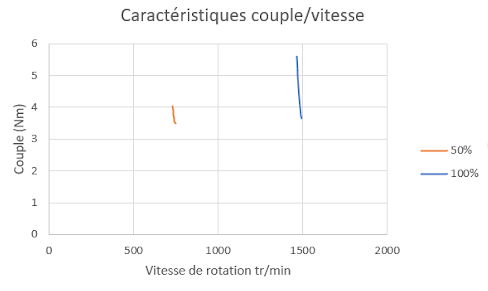
\includegraphics[width=12cm]{couple_vitesse2.png}
		\caption{Caractéristique couple/vitesse}
	\end{figure}

	Nous obtenons bien 2 courbes parallèles, ce résultat est en accord avec la théorie. Changer le rapport translate bien la courbe sur le graphe. Pour voir si les courbes sont bien en accord avec la théorie, il faudrait mesurer le couple maximum délivré qui devrait être le même pour les 2 courbes mais à 2 vitesses de rotation différentes.\\
	Avec ce mode d’alimentation, la machine peut fournir assez de couple pour fonctionner dans les deux cas avec une alimentation à 25 Hz ou à 50 Hz. La vitesse peut donc aller de 1450 à 1500 tr/min et de 725 à 750 tr/min.\\
	
	\subsection{Etude du régime dynamique - démarrage}
	
	Nous allons maintenant étudier le démarrage de la machine à vide sous ses différents modes d’alimentation à vitesse maximale. Pour ce faire, nous décalons la machine à courant continu. Nous relevons la réponse en courant et en vitesse de la machine.\\
	Nous alimentons d’abord la machine par le réseau : \\
	
	\begin{figure}[h]
		\centering
		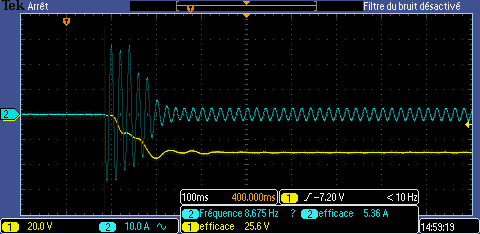
\includegraphics[width=12cm]{TEK00004.PNG}
		\caption{Alimentation directe}
	\end{figure}
	
	Nous pouvons voir un pic de courant allant jusqu’à presque 30 A. La vitesse de rotation maximale met environ 1 division soit un peu plus de 100 ms à s’établir, le courant se stabilise aussi à partir de cet instant. Avec un tel pic de courant, nous pouvons imaginer qu'en répétant un grand nombre de fois le démarrage de la machine, elle peut s’endommager. Ce système est certes très rapide mais il peut endommager la machine. Par exemple, ce mode d’alimentation ne serait pas adapté pour un ascenseur qui démarre souvent.\\
	Nous alimentons maintenant la machine par le variateur électronique dans le sens de rotation normal :\\
	
	\begin{figure}[h]
		\centering
		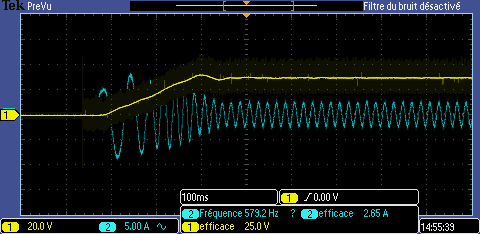
\includegraphics[width=12cm]{TEK00002.PNG}
		\caption{Alimentation variateur direction avant}
	\end{figure}
	\newpage
	
	Le système est cette fois plus lent à s’établir mais le pic de courant est beaucoup plus faible environ 7.5 A pour un temps de réponse d’environ 250 ms. Dans ce mode de fonctionnement, on dépasse le courant nominal de la machine, il y a même si il est plus faible que pour le cas précédent un risque d’usure de la machine. Ce mode n’est donc pas adapté pour le fonctionnement d’un ascenseur.\\
	
	Nous alimentons maintenant la machine par le variateur électronique dans le sens de rotation inverse :\\
	
	\begin{figure}[h]
		\centering
		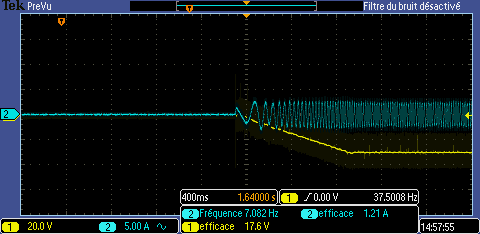
\includegraphics[width=12cm]{TEK00003.PNG}
		\caption{Alimentation variateur direction avant}
	\end{figure}
	\newpage
	Le démarrage a été programmé différemment, le système est beaucoup plus lent et met entre 800 et 900 ms à s’établir en revanche, il n’y a pas de pic de courant. Nous pouvons imaginer une utilisation ou la machine à besoin de redémarrer souvent avec cette programmation, il n’y aurait aucun danger d’usure lié au courant lors du démarrage. Cette alimentation serait bien adaptée pour un ascenseur.\\
	
	\section{Conclusion}
	
	Lors de ce TP, nous avons pu mettre en pratique les différentes méthodes de commandes vues en cours et nous avons comparé nos mesures avec la théorie.\\
	
	Nous avons bien pu noter l'efficacité de la commande en V/f qui permet bien de garder un couple suffisant pour entraîner l'ascenseur tout en cousommant un courant relativement faible, en effet avec la commande en tension simple, abaisser la tension à 190V a entraîné un courant trop grand pour que l'on puisse faire toute les mesures.
		
\end{document}